% Template for Cogsci submission with R Markdown

% Stuff changed from original Markdown PLOS Template
\documentclass[10pt, letterpaper]{article}

\usepackage{cogsci}
\usepackage{pslatex}
\usepackage{float}
\usepackage{caption}

% amsmath package, useful for mathematical formulas
\usepackage{amsmath}

% amssymb package, useful for mathematical symbols
\usepackage{amssymb}

% hyperref package, useful for hyperlinks
\usepackage{hyperref}

% graphicx package, useful for including eps and pdf graphics
% include graphics with the command \includegraphics
\usepackage{graphicx}

% Sweave(-like)
\usepackage{fancyvrb}
\DefineVerbatimEnvironment{Sinput}{Verbatim}{fontshape=sl}
\DefineVerbatimEnvironment{Soutput}{Verbatim}{}
\DefineVerbatimEnvironment{Scode}{Verbatim}{fontshape=sl}
\newenvironment{Schunk}{}{}
\DefineVerbatimEnvironment{Code}{Verbatim}{}
\DefineVerbatimEnvironment{CodeInput}{Verbatim}{fontshape=sl}
\DefineVerbatimEnvironment{CodeOutput}{Verbatim}{}
\newenvironment{CodeChunk}{}{}

% cite package, to clean up citations in the main text. Do not remove.
\usepackage{apacite}

% KM added 1/4/18 to allow control of blind submission
\cogscifinalcopy

\usepackage{color}

% Use doublespacing - comment out for single spacing
%\usepackage{setspace}
%\doublespacing


% % Text layout
% \topmargin 0.0cm
% \oddsidemargin 0.5cm
% \evensidemargin 0.5cm
% \textwidth 16cm
% \textheight 21cm

\title{Pressure to communicate across knowledge asymmetries leads to
pedagogically supportive language input}


\author{Benjamin C. Morris \and Daniel Yurovsky \\
        \texttt{\{benmorris, yurovsky\}@uchicago.edu} \\
       Department of Psychology \\ University of Chicago}

\begin{document}

\maketitle

\begin{abstract}
Children do not learn language from passive observation of the world,
but from interaction with caregivers who want to communicate with them.
These communicative exchanges are structured at multiple levels in ways
that support support language learning. We argue this pedagogically
supportive structure can result from pressure to communicate
successfully with a linguistically immature partner. We first
characterize one kind of pedagogically supportive structure in a corpus
analysis: caregivers provide more information-rich referential
communication, using both gesture and speech to refer to a single
object, when that object is rare and when their child is young. Then, in
an iterated reference game experiment on Mechanical Turk (n = 480), we
show how this behavior can arise from pressure to communicate
successfully with a less knowledgeable partner. Lastly, we show that
speaker behavior in our experiment can be explained by a rational
planning model, without any explicit teaching goal. We suggest that
caregivers' desire to communicate successfully may play a powerful role
in structuring children's input in order to support language learning.

\textbf{Keywords:}
language learning; communication; computational modeling.
\end{abstract}

\section{Introduction}\label{introduction}

One of the most striking aspects of children's language learning is just
how quickly they master the complex system of their natural language
(Bloom, 2000). In just a few short years, children go from complete
ignorance to conversational fluency in a way that is the envy of
second-language learners attempting the same feat later in life
(Newport, 1990). What accounts for this remarkable transition?

Distributional learning presents a unifying account of early language
learning: where infants come to language acquisition with a powerful
ability to learn the latent structure of language from the statistical
properties of speech in their ambient environment (Saffran, 2003). A
number of experiments clearly demonstrate the early availability of such
mechanisms and their utility across a range of language phenomena
(Saffran, 2003; Smith \& Yu, 2008). However, there is reason to be
suspicious about just how precocious young learners are early in
development. For example, infants' ability to track the co-occurrence
information connecting words to their referents appears to be highly
constrained by their developing memory and attention systems (Smith \&
Yu, 2013; Vlach \& Johnson, 2013). Further, computational models of
these processes show that the rate of acquisition is highly sensitive to
variation in environmental statistics (e.g., Vogt, 2012). Thus,
precocious unsupervised statistical learning appears to fall short of a
complete explanation for rapid early language learning.

Even relatively constrained statistical learning could be rescued,
however, if caregivers structured their language in a way that
simplified the learning problem. Indeed, evidence at a variety of
levels-- from speech segmentation to word learning-- suggests that
caregivers' naturalistic communication provides exactly this kind of
supportive structure (Gogate, Bahrick, \& Watson, 2000; Thiessen, Hill,
\& Saffran, 2005; Tomasello \& Farrar, 1986). Under distributional
learning accounts, the existence of this kind of structure is a
theory-external feature of the world that does not have an independently
motivated explanation. Indeed, because of widespread agreement that
parental speech is not usually motivated by explicit pedagogical goals,
the calibration of speech to learning mechanisms seems a happy accident;
parental speech just happens to be calibrated to children's learning
needs. In this work, we take the first steps toward a unifying account
of both the child's learning and the parents' production: Both are
driven by a pressure to communicate successfully (Brown, 1977).

Early, influential functionalist accounts of language learning focused
on the importance of communicative goals (e.g., Brown, 1977). Our goal
in this work is to formalize the intuitions in these accounts in a
computational model, and to test this model against experimental data.
We take as the caregiver's goal the desire to communicate with the
child, not about language itself, but instead about the world in front
of them. To succeed, the caregiver must produce the kinds of
communicative signals that the child can understand and respond
contingently, potentially leading caregivers to tune the complexity of
their speech as a byproduct of in-the-moment pressure to communicate
successfully (Yurovsky, 2017).

To examine this hypothesis, we first analyze parent communicative
behavior in a longitudinal corpus of parent-child interaction in the
home (Goldin-Meadow et al., 2014). We investigate the extent to which
parents tune their communicative behavior (focusing on modality--
i.e.~gesture vs.~speech) across their child's development to align to
their child's developing linguistic knowledge (Yurovsky, Doyle, \&
Frank, 2016). We take this phenomenon to be a case study of
pedagogically supportive structure in the language environment.

We then experimentally induce this form of structured language input in
a simple model system: an iterated reference game in which two players
earn points for communicating successfully with each other. Modeled
after our corpus data, participants are asked to make choices about
which communicative strategy to use (akin to modality choice). In an
experiment on Mechanical Turk using this model system, we show that
tuned, structured language input can arise from a pressure to
communicate. We then show that participant behavior in our game can be
explained by a rational planning model that seeks to optimize its total
expected utility over the course of the game.

\section{Corpus Analysis}\label{corpus-analysis}

We first investigate parent referential communication in a longitudinal
corpus of parent-child interaction. We analyze the production of
multi-modal cues (i.e.~using both gesture and speech) to refer to the
same object, in the same instance-- an information-rich cue that we take
as one instance of pedagogically supportive language input. While many
aspects of CDS support learning, multi-modal cues (e.g., speaking while
pointing or looking) are uniquely powerful sources of data for young
children (e.g., Baldwin, 2000). Multi-modal reference may be especially
pedagogically supportive if usage patterns reflect adaptive linguistic
tuning, with caregivers using this information-rich cue more for young
children and infrequent objects. The amount of multi-modal reference
should be sensitive to the child's age, such that caregivers will be
more likely to provide richer communicative information when their child
is younger (and has less linguistic knowledge) than as she gets older
(Yurovsky et al., 2016).

\subsection{Methods}\label{methods}

We used data from the Language Development Project-- a large-scale,
longitudinal corpus of parent child-interaction in the home with
families who are representative of the Chicago community in
socio-economic and racial diversity (Goldin-Meadow et al., 2014). These
data are drawn from a subsample of 10 families from the larger corpus.
Recordings were taken in the home every 4-months from when the child was
14-months-old until they were 34-months-old, resulting in 6 timepoints
(missing one family at the 30-month timepoint). Recordings were 90
minute sessions, and participants were given no instructions.

The Language Development Project corpus contains transcription of all
speech and communicative gestures produced by children and their
caregivers over the course of the 90-minute home recordings. An
independent coder analyzed each of these communicative instances and
identified each time a concrete noun was referenced using speech (in
specific noun form), gesture (only deictic gestures were coded for ease
of coding and interpretation-- e.g., pointing) or both simultaneously.

\subsection{Results}\label{results}

These corpus data were analyzed using a mixed effects regression to
predict parent use of multi-modal reference for a given referent. Random
effects of subject and referent were included in the model. Our key
predictors were child age and logged referent frequency (i.e.~how often
a given object was referred to overall across our data).

We find a significant negative effect of child age (in months) on
multi-modal reference, such that parents are significantly less likely
to produce the multi-modal cue as their child gets older (\emph{B =}
-0.04, \emph{p \textless{} 0.0001}). We also find a significant negative
effect of referent frequency on multi-modal reference as well, such that
parents are significantly less likely to provide the multi-modal cue for
frequent referents than infrequent ones (\emph{B =} -0.13, \emph{p
\textless{} 0.0001}). Thus, in these data, we see early evidence that
parents are providing richer, structured input about rarer things in the
world for their younger children.

\begin{CodeChunk}
\begin{figure}[tb]

{\centering 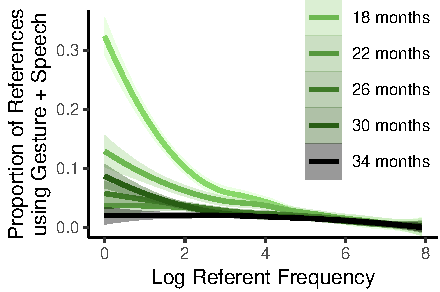
\includegraphics{figs/corpus_plot-1} 

}

\caption[Proportion of parent multi-modal referential talk across development]{Proportion of parent multi-modal referential talk across development. The log of a referent's frequency is given on the x-axis, with less frequent items closer to zero.}\label{fig:corpus_plot}
\end{figure}
\end{CodeChunk}

\subsection{Discussion}\label{discussion}

Caregivers are not indiscriminate in their use of multi-modal reference;
in these data, they provided more of this support when their child was
younger and when discussing less familiar objects. These longitudinal
corpus findings are consistent with an account of parental alignment:
parents are sensitive to their child's linguistic knowledge and adjust
their communication accordingly (Yurovsky et al., 2016). Ostensive
labeling is perhaps the most explicit form of pedagogical support, so we
chose to focus on it for our first case study. We argue that these data
could be explained by a simple, potentially-selfish pressure: to
communicate successfully. The influence of communicative pressure is
difficult to draw in naturalistic data, so we developed a paradigm to
try to experimentally induce richly-structured, aligned input from a
pressure to communicate in the moment.

\section{Experimental Framework}\label{experimental-framework}

We developed a simple reference game in which participants would be
motivated to communicate successfully on a trial-by-trial basis. In all
conditions, participants were placed in the role of speaker and asked to
communicate with a computerized listener whose responses were programmed
to be contingent on speaker behavior. We manipulated the relative costs
of the communicative methods (gesture and speech) across conditions, as
we did not have a direct way of assessing these costs in our
naturalistic data, and they may vary across communicative contexts. In
all cases, we assumed that gesture was more costly than speech. Though
this need not be the case for all gestures and contexts, our framework
compares simple lexical labeling and unambiguous deictic gestures, which
likely are more costly and slower to produce (see Yurovsky, Meyers,
Burke, \& Goldin-Meadow, 2018). We also established knowledge
asymmetries by pre-training participants and manipulating how much
training they thought their partner received. Using these manipulations,
we aimed to experimentally determine the circumstances under which
richly-structured input emerges, without an explicit pedagogical goal.

\subsection{Method}\label{method}

\subsubsection{Participants}\label{participants}

480 participants were recruited though Amazon Mechanical Turk and
received \$1 for their participation. Data from 51 participants were
excluded from subsequent analysis for failing the critical manipulation
check and a further 28 for producing pseudo-English labels (e.g.,
`pricklyyone'). The analyses reported exclude the data from those
participants, but all analyses were also conducted without excluding any
participants and all patterns hold (\emph{ps \textless{} 0.05}).

\subsubsection{Design and Procedure}\label{design-and-procedure}

Participants were exposed to nine novel objects, each with a randomly
assigned pseudo-word label. We manipulated the exposure rate
within-subjects: during training participants saw three of the nine
object-label mappings four times, two times, or one time. Participants
were then given a recall task to establish their knowledge of the novel
lexicon (pretest).

\begin{CodeChunk}
\begin{figure}[tb]

{\centering 
\includegraphics{figs/exp_screenshot-1} 

}

\caption[Screenshot of speaker view during gameplay]{Screenshot of speaker view during gameplay.}\label{fig:exp_screenshot}
\end{figure}
\end{CodeChunk}

Prior to beginning the game, participants are told how much exposure
their partner has had to the lexicon and also that they will be asked to
discuss each object three times. As a manipulation check, participants
are then asked to report their partner's level of exposure, and are
corrected if they answer wrongly. Then during gameplay, speakers saw a
target object in addition to an array of all nine objects (see Figure
\ref{fig:exp_screenshot} for the speaker's perspective). Speakers had
the option of either directly click on the target object in the array
(gesture)- a higher cost cue but without ambiguity- or typing a label
for the object (speech)- a lower cost cue but contingent on the
listener's shared linguistic knowledge. After sending the message,
speakers are shown which object the listener selected.

Speakers could win up to 100 points per trial if the listener correctly
selected the target referent. We manipulated the relative utility of the
speech cue between-subjects across two conditions: low relative cost for
speech (`Low Relative Cost') and higher relative cost for speech
(`Higher Relative Cost'). In the `Low Relative Cost' condition, speakers
were charged 70 points for gesturing and 0 points for labeling, yielding
30 points and 100 points respectively if the listener selected the
target object. In the `Higher Relative Cost' condition, speakers were
charged 50 points for gesturing and 20 points for labeling, yielding up
to 50 points and 80 points respectively. If the listener failed to
identify the target object, the speaker nevertheless paid the relevant
cost for that message in that condition. As a result of this
manipulation, there was a higher relative expected utility for labeling
in the `Low Relative Cost' condition than the `Higher Relative Cost'
condition.

Critically, participants were told about a third type of possible
message using both gesture and speech within a single trial to
effectively teach the listener an object-label mapping. This action
directly mirrors the multi-modal reference behavior from our corpus
data-- it presents the listener with an information-rich, potentially
pedagogical learning moment. In order to produce this teaching behavior,
speakers had to pay the cost of producing both cues (i.e.~both gesture
and speech). Note that, in all utility conditions, teaching yielded
participants 30 points (compared with the much more beneficial strategy
of speaking which yielded 100 points or 80 points across our two utility
manipulations).

To explore the role of listener knowledge, we also manipulated
participants' expectations about their partner's knowledge across 3
conditions. Participants were told that their partner had either no
experience with the lexicon, had the same experience as the speaker, or
had twice the experience of the speaker.

Listeners were programmed with starting knowledge states initialized
accordingly. Listeners with no exposure began the game with knowledge of
0 object-label pairs. Listeners with the same exposure of the speaker
began with knowledge of five object-label pairs (3 high frequency, 1 mid
frequency, 1 low frequency), based the average retention rates found
previously. Lastly, the listener with twice as much exposure as the
speaker began with knowledge of all nine object-label pairs. If the
speaker produced a label, the listener was programmed to consult their
own knowledge of the lexicon and check for similar labels (selecting a
known label with a Levenshtein edit distance of two or fewer from the
speaker's production), or select among unknown objects if no similar
labels are found. Listeners could integrate new words into their
knowledge of the lexicon if taught.

Crossing our 2 between-subjects manipulations yielded 6 conditions (2
utility manipulations: `Low Relative Cost' and `Higher Relative Cost';
and 3 levels of partner's exposure: None, Same, Double), with 80
participants in each condition. We expected to find results that
mirrored our corpus findings such that rates of teaching would be higher
when there was an asymmetry in knowledge where the speaker knew more
(None manipulation) compared with when there was equal knowledge (Same
manipulation) or when the listener was more familiar with the language
(Double manipulation). We expected that participants would also be
sensitive to our utility manipulation, such that rates of labeling and
teaching would be higher in the `Low Relative Cost' conditions than the
other conditions.

\subsection{Results}\label{results-1}

As an initial check of our exposure manipulation, a logistic regression
showed that participants were significantly more likely to recall the
label for objects with two exposures (\emph{B =} 1.66, \emph{p
\textless{} 0.0001}) or with four exposures (\emph{B =} 3.07, \emph{p
\textless{} 0.0001}), compared with objects they saw only once. On
average, participants knew at least 6 of the 9 words in the lexicon
(mean = 6.28, sd = 2.26).

\subsubsection{Gesture-Speech Tradeoff.}\label{gesture-speech-tradeoff.}

To determine how gesture and speech are trading off across conditions,
we looked at a mixed effects logistic regression to predict whether
speakers chose to produce a label during a given trial as a function of
the exposure rate, object instance in the game (first, second, or
third), utility manipulation, and partner manipulation. A random
subjects effects term was included in the model. There was a significant
effect of exposure rate such that there was more labeling for objects
with two exposures (\emph{B =} 0.91, \emph{p \textless{} 0.0001}) or
with four exposures (\emph{B =} 1.83, \emph{p \textless{} 0.0001}),
compared with objects seen only once at training. Compared with the
first instance of an object, speakers were significantly more likely to
produce a label on the second appearance (\emph{B =} 0.2, \emph{p
\textless{} 0.01}) or third instance of a given object (\emph{B =} 0.46,
\emph{p \textless{} 0.0001}). Participants also modulated their
communicative behavior on the basis of the utility manipulation and our
partner exposure manipulation. Speakers in the Low Relative Cost
condition produced significantly more labels than participants in the
Higher Relative Cost condition (\emph{B =} -0.84, \emph{p \textless{}
0.001}). Speakers did more labeling with more knowledgeable partners;
compared with the listener with no exposure, there were significantly
higher rates of labeling in the same exposure (\emph{B =} 1.74, \emph{p
\textless{} 0.0001}) and double exposure conditions (\emph{B =} 3.14,
\emph{p \textless{} 0.001}).

\begin{CodeChunk}
\begin{figure}[tb]

{\centering 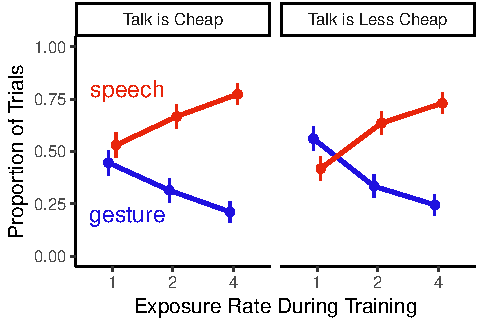
\includegraphics{figs/exp_speech_gesture-1} 

}

\caption[Speaker communicative method choice as a function of exposure and the utility manipulation]{Speaker communicative method choice as a function of exposure and the utility manipulation. Data are taken from the Double Exposure manipulation. Rates of teaching were minimal and are not shown.}\label{fig:exp_speech_gesture}
\end{figure}
\end{CodeChunk}

Figure \ref{fig:exp_speech_gesture} illustrates the gesture-speech
tradeoff pattern in the Double Exposure condition (as there was minimal
teaching in that condition, so the speech-gesture trade-off is most
interpretable). The effects on gesture mirror those found for labeling
and are thus not included for brevity (\emph{ps \textless{} 0.01}). Note
that these effects cannot be explained by participant knowledge; all
patterns above hold when looking \emph{only} at words known by the
speaker at pretest (\emph{ps \textless{} 0.01}). Further, these patterns
directly mirror previous corpus analyses demonstrating the
gesture-speech tradeoff in naturalistic parental communicative
behaviors, where lexical knowledge is likely for even the least frequent
referent (see Yurovsky et al., 2018).\\
\newline

\subsubsection{Emergence of Teaching.}\label{emergence-of-teaching.}

In line with our hypotheses, a mixed effects logistic regression
predicting whether or not teaching occurred on a given trial revealed
that teaching rates across conditions depend on all of the same factors
that predict speech and gesture (see Figure \ref{fig:exp_teach}). There
was a significant positive effect of initial training on the rates of
teaching, such that participants were more likely to teach words with
two exposures (\emph{B =} 0.26, \emph{p \textless{} 0.05}) and four
exposures (\emph{B =} 0.25, \emph{p \textless{} 0.05}), compared with
words seen only once at training. There was also a significant effect of
the utility manipulation such that being in the Low Relative Cost
condition predicted higher rates of teaching than being in the Higher
Relative Cost condition (\emph{B =} -0.96, \emph{p \textless{} 0.001}),
a rational response considering teaching allows one to use a less costly
strategy in the future and that strategy is especially superior in the
Low Relative Cost condition.

We found an effect of partner exposure on rates of teaching as well:
participants were significantly more likely to teach a partner with no
prior exposure to the language than a partner with the same amount of
exposure as the speaker (\emph{B =} -1.63, \emph{p \textless{} 0.0001})
or double their exposure (\emph{B =} -3.51, \emph{p \textless{}
0.0001}). The planned utility of teaching comes from using another,
cheaper strategy (speech) on later trials, thus the expected utility of
teaching should decrease when there are fewer subsequent trials for that
object, predicting that teaching rates should drop dramatically across
trials for a given object. Compared with the first trial for an object,
speakers were significantly less likely to teach on the second trial
(\emph{B =} -0.84, \emph{p \textless{} 0.0001}) or third trial (\emph{B
=} -1.67, \emph{p \textless{} 0.0001}).

\subsection{Discussion}\label{discussion-1}

As predicted, the data from our paradigm corroborate our findings from
the corpus analysis, demonstrating that pedagogically supportive
behavior emerges despite the initial cost when there is an asymmetry in
knowledge and when speech is less costly than other modes of
communication. While this paradigm has stripped away much of the
interactive environment of the naturalistic corpus data, it provides
important proof of concept that the structured and tuned language input
we see in those data could arise from a pressure to communicate. The
paradigm's clear, quantitative predictions also allow us to build a
formal model to predict our empirical results.

\begin{CodeChunk}
\begin{figure}[tb]
\includegraphics{figs/exp_teach-1} \caption[Rates of teaching across the 6 conditions, plotted by how many times an object had been the target object]{Rates of teaching across the 6 conditions, plotted by how many times an object had been the target object.}\label{fig:exp_teach}
\end{figure}
\end{CodeChunk}

\section{Model: Communication as
planning}\label{model-communication-as-planning}

The results from this experiment are qualitatively consistent with a
model in which participants make their communicative choices to maximize
their expected utility from the reference game. We next formalize this
model to determine if these results are predicted quantitatively as
well.

\newcommand{\E}[1]{\mathbb{E}\left[ #1 \right]}

We take as inspiration the idea that communication is a kind of
action--e.g.~talking is a speech act (Austin, 1975). Consequently, we
can understand the choice of \emph{which communicative act} a speaker
should take as a question of which act would maximize their utility:
achieving successful communication while minimizing their cost (Frank \&
Goodman, 2012). In this game, speakers can take three actions: talking,
pointing, or teaching. In this reference game, these Utilities (\(U\))
are given directly by the rules. Because communication is a repeated
game, people should take actions that maximize their Expected Utility
(\(EU\)) over the course of not just this act, but all future
communicative acts with the same conversational partner. We can think of
communication, then as a case of recursive planning. However, people do
not have perfect knowledge of each-other's vocabularies (\(v\)).
Instead, they only have uncertain beliefs (\(b\)) about these
vocabularies that combine their expectations about what kinds of words
people with as much linguistic experience as their partner are likely to
know with their observations of their partner's behavior in past
communicative interactions. This makes communication a kind of planning
under uncertainty well modeled as a Partially Observable Markov Decision
Process (POMDP, Kaelbling, Littman, \& Cassandra, 1998).

Optimal planning in a POMDP involves a cycle of four phases: (1) Plan,
(2) Act, (3) Observe, (4) Update beliefs. When people plan, they compute
the Expected Utility of each possible action (\(a\)) by combining the
Expected Utility of that action now with the Discounted Expected Utility
they will get in all future actions. The amount of discounting
(\(\gamma\)) reflects how people care about success now compared to
success in the future. In our simulations, we set \(\gamma=.5\) in line
with prior work. Because Utilities depend on the communicative partner's
vocabulary, people should integrate over all possible vocabularies in
proportion to the probability that their belief assigns to that
(\(\mathbb{E}_{v \sim b}\)). \[
EU\left[a\right | b] = \mathbb{E}_{v \sim b} \left(U(a|v) + \gamma \,\mathbb{E}_{v',o',a'} \,\left( EU\left[a' | b'\right]\right)\right)
\] Next, people take an action as a function of its Expected Utility.
Following other models in the Rational Speech Act framework, we use the
Luce Choice Axiom, in which each choice is taken in probability
proportional to its exponentiated utility (Frank \& Goodman, 2012; Luce,
1959). This choice rule has a single parameter \(\alpha\) that controls
the noise in this choice--as \(\alpha\) approaches 0, choice is random
and as \(\alpha\) approaches infinity choice is optimal. For the results
reported here, we set \(\alpha = 2\) based on hand-tuning, but other
values produce similar results. \[ 
P\left(a|b\right) \propto \alpha \, e^{EU[a|b]}
\]

After taking an action, people observe (\(o\)) their partner's
choice--sometimes they pick the intended object, and sometimes they
don't. They then update their beliefs about the partner's vocabulary
based on this observation. For simplicity, we assume that people think
their partner should always select the correct target if they point to
it, or if they teach, and similarly should always select the correct
target if they produce its label and the label is in their partner's
vocabulary. Otherwise, they assume that their partner will select the
wrong object. People could of course have more complex inferential
rules, e.g.~assuming that if their partner does know a word they will
choose among the set of objects whose labels they do not know (mutual
exclusivity, Markman \& Wachtel, 1988). Empirically, however, our simple
model appears to accord well with people's behavior. \[
b'(v') \propto P\left(o|v',a\right) \sum_{v \in V}P\left(v'|v,a\right)b\left(v\right)
\]

The critical feature of a repeated communication game is that people can
change their partner's vocabulary. In teaching, people pay the cost of
both talking and pointing together, but can leverage their partner's new
knowledge on future trials. Note here that teaching has an upfront cost
and the only benefit to be gained comes from using less costly
communication modes later. There is no pedagogical goal-- the model
treats speakers as selfish agents aiming to maximize their own utilities
by communicating successfully. We assume for simplicity that learning is
approximated by a simple Binomial learning model. If someone encounters
a word \(w\) in an unambiguous context (e.g.~teaching), they add it to
their vocabulary with probability \(p\). We also assume that over the
course of this short game that people do not forget--words that enter
the vocabulary never leave, and that no learning happens by inference
from mutual exclusivity.

\[
P\left(v'|v,a\right)= \begin{cases} 
1 & \text{if } v_{w} \in v \& v'\\ 
p & \text{if } v_{w} \notin v \& a = \text{point+talk}\\ 
0 & otherwise\end{cases}
\]

The final detail is to specify how people estimate their partner's
learning rate (\(p\)) and initial vocabulary (\(v\)). We propose that
people begin by estimating their own learning rate by reasoning about
the words they learned at the start of the task: Their \(p\) is the rate
that maximizes the probability of them having learned their initial
vocabularies from the trials they observed. People can then expect their
partner to have a similar \(p\) (per the ``like me'' hypothesis,
Meltzoff, 2005). Having an estimate of their partner's \(p\), they can
estimate their vocabulary by simulating their learning from the amount
of training we told them their partner had before the start of the game.

\subsection{Model Results}\label{model-results}

The fit between our model's predictions and our empirical data from our
reference game study on Amazon Turk can be seen in Figure
\ref{fig:model_fit}. The model outputs trial-level action predictions
(e.g., ``speak'') for every speaker in our empirical data. These model
outputs were aggregated across the same factors as the empirical data:
modality, appearance, partner's exposure, and utility condition. We see
a significant correlation of our model predictions and our empirical
data (\emph{r = 0.94, p\textless{}0.0001}). Our model provides a strong
fit for these data, supporting our conclusion that richly-structured
language input could emerge from in-the-moment pressure to communicate,
without a goal to teach.

\begin{CodeChunk}
\begin{figure}[H]

{\centering 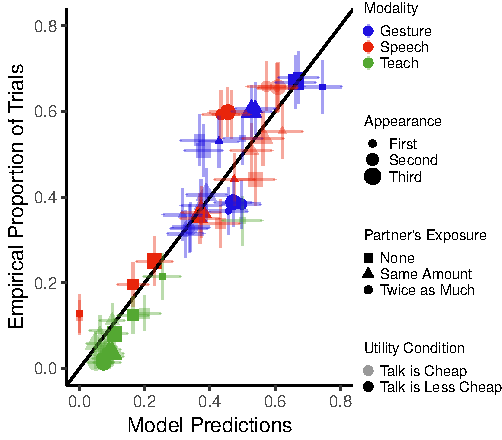
\includegraphics{figs/model_fit-1} 

}

\caption[Fit between model predictions and empirical data]{Fit between model predictions and empirical data.}\label{fig:model_fit}
\end{figure}
\end{CodeChunk}

\section{General Discussion}\label{general-discussion}

We showed that people tune their communicative choices to varying cost
and reward structures, and also critically to their partner's linguistic
knowledge--providing richer cues when partners are unlikely to know
language and many more rounds remain. These data are consistent with the
patterns shown in our corpus analysis of parent referential
communication and demonstrate that such pedagogically supportive input
could arise from a motivation to maximize communicative success while
minimizing communicative cost-- no additional motivation to teach is
necessary. Our account is not specific to any particular language
phenomenon, though we have focused on multi-modal reference here. Given
the right data or paradigm, our account should hold equally well when
explaining how other information-rich language input could arise.

Of course, many aspects of language do not differ in speech to children
(e.g., syntax, see Newport, Gleitman, \& Gleitman, 1977). On our
account, not all aspects of language should be calibrated to child's
language development--only those that support communication. A full
account that explains variability in modification across aspects of
language will rely on a fully specified model of optimal communication.
Such a model will allow us to determine both which structures are
predictably unmodified, and which structures must be modified for other
reasons. Nonetheless, this work is an important first step in validating
the hypothesis that language input that is structured to support
language learning could arise from a single unifying goal: The desire to
communicate effectively.

\vspace{1em}\fbox{ \parbox[b][][c]{7.5cm}{\centering The Mechanical Turk experiment was preregistered on Open Science Framework at https://osf.io/63qdg All data and code for analyses are available at https://github.com/benjamincmorris/reference-game \ }}

\section{Acknowledgements}\label{acknowledgements}

This research was funded by a James S. McDonnell Foundation Scholar
Award to DY.

\section{References}\label{references}

\setlength{\parindent}{-0.1in} \setlength{\leftskip}{0.125in}

\noindent

\hypertarget{refs}{}
\hypertarget{ref-austin1975}{}
Austin, J. L. (1975). \emph{How to do things with words} (Vol. 88).
Oxford university press.

\hypertarget{ref-baldwin2000}{}
Baldwin, D. (2000). Interpersonal understanding fuels knowledge
acquisition. \emph{Current Directions in Psychological Science},
\emph{9}, 40--45.

\hypertarget{ref-bloom2000}{}
Bloom, P. (2000). \emph{How children learn the meanings of words}. MIT
press: Cambridge, MA.

\hypertarget{ref-brown1977}{}
Brown, R. (1977). Introduction. In C. E. Snow \& C. A. Ferguson (Eds.),
\emph{Talking to children: Language input and interaction}. Cambridge,
MA.: MIT Press.

\hypertarget{ref-frank2012}{}
Frank, M. C., \& Goodman, N. D. (2012). Predicting pragmatic reasoning
in language games. \emph{Science}, \emph{336}(6084), 998--998.

\hypertarget{ref-gogate2000}{}
Gogate, L. J., Bahrick, L. E., \& Watson, J. D. (2000). A study of
multimodal motherese: The role of temporal synchrony between verbal
labels and gestures. \emph{Child Development}, \emph{71}(4), 878--894.

\hypertarget{ref-goldin-meadow2014}{}
Goldin-Meadow, S., Levine, S. C., Hedges, L. V., Huttenlocher, J.,
Raudenbush, S. W., \& Small, S. L. (2014). New evidence about language
and cognitive development based on a longitudinal study: Hypotheses for
intervention. \emph{American Psychologist}, \emph{69}(6), 588--599.

\hypertarget{ref-kaelbling1998}{}
Kaelbling, L. P., Littman, M. L., \& Cassandra, A. R. (1998). Planning
and acting in partially observable stochastic domains. \emph{Artificial
Intelligence}, \emph{101}, 99--134.

\hypertarget{ref-luce1959}{}
Luce, R. D. (1959). Individual choice behavior.

\hypertarget{ref-markman1988}{}
Markman, E. M., \& Wachtel, G. F. (1988). Children's use of mutual
exclusivity to constrain the meanings of words. \emph{Cognitive
Psychology}, \emph{20}(2), 121--157.

\hypertarget{ref-meltzoff2005}{}
Meltzoff, A. N. (2005). Imitation and other minds: The ``like me''
hypothesis. \emph{Perspectives on Imitation: From Neuroscience to Social
Science}, \emph{2}, 55--77.

\hypertarget{ref-newport1990}{}
Newport, E. L. (1990). Maturational constraints on language learning.
\emph{Cognitive Science}, \emph{14}(1), 11--28.

\hypertarget{ref-newport1977}{}
Newport, E. L., Gleitman, H., \& Gleitman, L. R. (1977). Mother, I'd
rather do it myself: Some effects and non-effects of maternal speech
style. In C. A. Ferguson (Ed.), \emph{Talking to children language input
and interaction} (pp. 109--149). Cambridge University Press.

\hypertarget{ref-saffran2003}{}
Saffran, J. R. (2003). Statistical language learning: Mechanisms and
constraints. \emph{Current Directions in Psychological Science},
\emph{12}(4), 110--114.

\hypertarget{ref-smith2008}{}
Smith, L. B., \& Yu, C. (2008). Infants rapidly learn word-referent
mappings via cross-situational statistics. \emph{Cognition}, \emph{106},
1558--1568.

\hypertarget{ref-smith2013}{}
Smith, L. B., \& Yu, C. (2013). Visual attention is not enough:
Individual differences in statistical word-referent learning in infants.
\emph{Language Learning and Development}, \emph{9}, 25--49.

\hypertarget{ref-thiessen2005}{}
Thiessen, E., Hill, E. A., \& Saffran, J. R. (2005). Infant-directed
speech facilitates word segmentation. \emph{Infancy}, \emph{7}, 53--71.

\hypertarget{ref-tomasello1986}{}
Tomasello, M., \& Farrar, M. J. (1986). Joint attention and early
language. \emph{Child Development}, \emph{57}(6), 1454--1463.

\hypertarget{ref-vlach2013}{}
Vlach, H. A., \& Johnson, S. P. (2013). Memory constraints on infants
cross-situational statistical learning. \emph{Cognition}, \emph{127}(3),
375--382.

\hypertarget{ref-vogt2012}{}
Vogt, P. (2012). Exploring the robustness of cross-situational learning
under zipfian distributions. \emph{Cognitive Science}, \emph{36}(4),
726--739.

\hypertarget{ref-yurovsky2017}{}
Yurovsky, D. (2017). A communicative approach to early word learning.
\emph{New Ideas in Psychology}, 1--7.

\hypertarget{ref-yurovsky2016}{}
Yurovsky, D., Doyle, G., \& Frank, M. C. (2016). Linguistic input is
tuned to childrens developmental level. In \emph{Proceedings of the
annual meeting of the cognitive science society} (pp. 2093--2098).

\hypertarget{ref-yurovsky2018}{}
Yurovsky, D., Meyers, M., Burke, Nicole, \& Goldin-Meadow, S. (2018).
Children gesture when speech is slow to come. In \emph{Proceedings of
the annual meeting of the cognitive science society} (pp. 2765--2770).

\bibliographystyle{apacite}


\end{document}
